\chapter{PROPOSED SOLUTION}
\label{chap:solution}

This chapter describes the team's solution overview and details of each component. In the overview, this report briefly describe the system as a whole and in the other sections, details of each component is defined in a clearer way.
\section{System overview}
\subsection{Requirement analysis}
As mentioned in \ref{introduction},
Figure \ref{chap3:system_overview_basic} shows an brief overview of how the system operate. Users interact with this system through \textbf{User Interfaces}
. Input of users can come in the form of images, videos or label contribution. The whole operational logic of the  system is contained within a \textbf{Crowd-sourcing server}. The server takes input of users and store them in database. It also loads appropriate contents from database and show users through user interfaces. 
\begin{center}
    \begin{figure}[H]
    \centering
    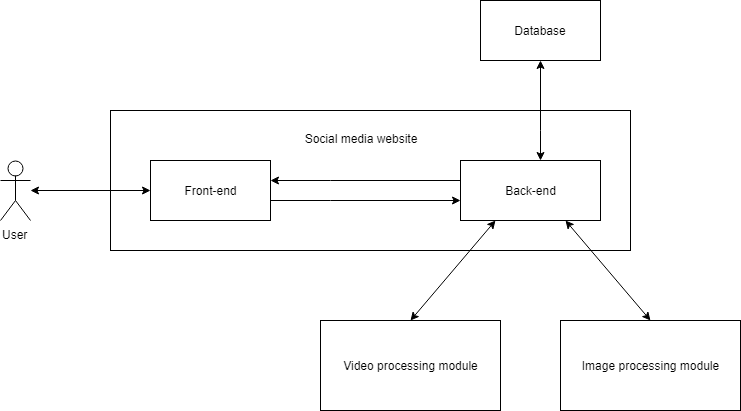
\includegraphics[width=1\columnwidth]{images/chap3/system_overview_basic.png}
    \footcaption{An overview of the system}
    \label{chap3:system_overview_basic}
    \end{figure}
\end{center}
Whenever there is a video to analyze,the server will send it to the \textbf{Video classifier module}, then get the results back. Results returned from video classifier module are classified activity from the video and frames that contain faces in them. \textbf{Face Recognition module} does the job of identifying people in images. Results of both \textbf{Video classifier module} and \textbf{Face Recognition module} are used to determine security threats each video or image shows.

\section{Crowd-sourcing system}
\subsection{Database}
\section{Classifier modules}
The project requires two systems for analysis: A face recognition system and a video classifier system. The facial recognition system takes pictures of human faces as input and return their identification. The video classifier system analyzes videos to find out actions in them. The remaining of this section describes in detail about the two analysis system.
\subsection{Face recognition system}

\subsection{Video classifier system}
